% Compile with:
% latexmk -pdf -pvc -interaction=nonstopmode
%\documentclass[aspectratio=169,10pt,draft]{beamer}
\documentclass[aspectratio=169,10pt]{beamer}

\usetheme{UniBern}
\title{Welcome \& Hello!}
\author{David Haberthür}
\institute{Institute of Anatomy\\University of Bern\\Switzerland}
\date{October 21, 2019 | \href{https://ilias.unibe.ch/goto_ilias3_unibe_crs_1589464.html}{MicroCT Workshop}}

%\includeonlyframes{current}
%then....
%\begin{frame}[label=current]
%\end{frame}

\usepackage{microtype}
\usepackage[backend=biber,
	style=numeric,
	url=false,
	isbn=true,
	maxbibnames=1,
	maxcitenames=1,
	sorting=none]{biblatex}
	\addbibresource{../../Documents/library.bib}
\usepackage{graphicx}
\usepackage{tikz}
\usepackage{pgfplots}
	\pgfplotsset{compat=newest}
\usepackage[detect-all=true,
	range-phrase=--,
	range-units=single,
	binary-units=true,
	per-mode=symbol,
	per-symbol=/]{siunitx}
\usepackage[absolute,
	overlay]{textpos} %for the \source{} command
\usepackage{gitinfo2}
\usepackage[version=4]{mhchem}
\usepackage{xspace}
\usepackage{ccicons}
\usepackage{animate}
\usepackage{listings}
	\lstset{frame=single,
		%backgroundcolor = \color{lightgray},
		basicstyle=\tiny\ttfamily
		}
\usepackage{tcolorbox}		
\usepackage{fontawesome5}
\usepackage{csquotes}

% change tikz font to slide font
% https://tex.stackexchange.com/a/33329/828
\usepackage[eulergreek]{sansmath}
\pgfplotsset{tick label style = {font=\sansmath\sffamily},
	every axis label = {font=\sansmath\sffamily},
	legend style = {font=\sansmath\sffamily},
	label style = {font=\sansmath\sffamily}
	}

% Globally thicker lines in with tikz
% https://tex.stackexchange.com/a/206769/828
\tikzset{every picture/.style={semithick}}

% And thicker plots by default
% https://tex.stackexchange.com/a/235439/828
% https://tex.stackexchange.com/q/262486/828
\pgfplotsset{%
	every axis plot/.append style={semithick},
	every axis/.append style={semithick}
	every axis plot post/.append style={every mark/.append style={semithick}}
	}

% stripped-down plot styling
% Based on https://tex.stackexchange.com/a/155210/828
% And then start each plot with `\begin{axis}[tuftelike,'
\pgfkeys{%
	/pgfplots/simplified/.style={%
		tick style={major tick length=0pt},
%		separate axis lines,
%		axis x line*=bottom,
%		axis x line shift=10pt,
%		xlabel shift=1pt,
%		axis y line*=left,
%		axis y line shift=10pt,
		ymajorgrids=true,
		axis line style={draw=none},
%		ylabel shift=1pt
		}
	}

% Some often used abbreviations
\newcommand{\imsize}{\linewidth} % set global image width
\newcommand{\everyframe}{1} % use only every nth frame for the movies
\newlength\imagewidth % needed for scalebars
\newlength\imagescale % needed for scalebars
\newcommand{\uct}{\si{\micro}CT\xspace} % make our life easier

% Acknowledge images just below them
% Based on https://tex.stackexchange.com/a/282637
\newcommand{\source}[2]{%
	\raisebox{-1.618ex}{\makebox[0pt][r]{\scriptsize\href{http://#1}{#1} #2}}
}

% Define us our custom footer
% Footer alignment with the help of https://tex.stackexchange.com/a/398534/828
% The alignment is not pixel-perfect, but good enough
% See for yourself by uncommenting the next line
%\setbeamercolor*{footline}{fg=orange,bg=ubRed} 
\defbeamertemplate{footline}{unibe}{%
	\begin{beamercolorbox}[wd=\paperwidth,sep=2pt]{footline}%
		\hspace*{\fill}%
		v. \href{https://github.com/habi/Talk.2019.MicroCTWorkshop/commit/\gitHash}{\gitAbbrevHash}\xspace|\xspace%
		p.\xspace\insertframenumber/\inserttotalframenumber%
		\hspace*{2pt}%
	\end{beamercolorbox}%
}%
\setbeamertemplate{footline}[unibe]

% Format bibliography for beamer
% http://tex.stackexchange.com/a/10686/828
\renewbibmacro{in:}{}
% http://tex.stackexchange.com/a/13076/828
\AtEveryBibitem{%
	\clearfield{journaltitle}
	\clearfield{pages}
	\clearfield{volume}
	\clearfield{number}
	\clearname{editor}
	\clearfield{issn}
	\clearfield{year}
}
% No parentheses around the (now empty) year: https://tex.stackexchange.com/a/147537
\renewcommand{\bibopenparen}{\addcomma\addspace}
\renewcommand{\bibcloseparen}{\addcomma\addspace}

% Slide transiton
%\addtobeamertemplate{background canvas}{\transfade[duration=0.5]}{}

% open in fullscreen
%\hypersetup{pdfpagemode=FullScreen}

% Move the text down a bit
% THIS IS A BIG HACK, IT SHOULD BE FIXED IN THE TEMPLATE
\addtobeamertemplate{frametitle}{}{\vspace*{1.5ex}}

\begin{document}
% No footline on the title page
% http://tex.stackexchange.com/a/18829/828 helps us to achieve that
{%
	\setbeamertemplate{footline}{}%
	\frame{\titlepage}%
}

\begin{frame}{WiFi}
	\begin{itemize}
		\item Use \emph{\href{https://www.eduroam.org/}{eduroam}}
		\item Or connect to \emph{public-unibe}
		\begin{itemize}
			\item Select the menu item \emph{Guest Login}
			\item Register with your mobile number and the voucher code
			\begin{tcolorbox}[width=3.3cm,colframe=ubRed,colback=ubGrey,halign=center,halign title=center,title=Voucher code]
				% Get the currently valid guest voucher here: https://idos-wiki.unibe.ch/vouchers
				\input{voucher}
			\end{tcolorbox}
			\item You will receive your access code by SMS
		\end{itemize}
	\end{itemize}	
\end{frame}

\begin{frame}{Tuesday lunch}
\centering
\huge
Choose your \faPizzaSlice

Go to \href{https://doodle.com/poll/6ci4dvpr88wvzwzn}{small.cat/low} \& mark your preference
\end{frame}

\begin{frame}
	\frametitle{Hello!}
	\begin{itemize}
		\item<1-> University of Bern, Switzerland
		\item<1-> Institute of Anatomy
		\item<1-> \uct-group: Ruslan Hlushchuk, David Haberthür, Oleksiy-Zakhar Khoma, Fluri Wieland, Carlos Correa Shokiche
		\item<1-> Biomedical research
		\begin{itemize}
			\item microangioCT~\cite{Hlushchuk2018}: Tumor vasculature, angiogenesis in the heart, musculature and bones
			\item Cancer research: Melanoma
			\item Lung imaging: Tumor detection and classification
			\item Physiology: Zebrafish musculature and gills~\cite{Messerli2019a}
		\end{itemize}
		\item<1-> SkyScan 1172 \& 1272 \uncover<2->{\& 2214}
	\end{itemize}
\end{frame}

\begin{frame}
	\frametitle{Gill anatomy}
	\centering
	% Image adapted from https://teacheratsea.files.wordpress.com/2011/07/gills-an-o2.jpg
	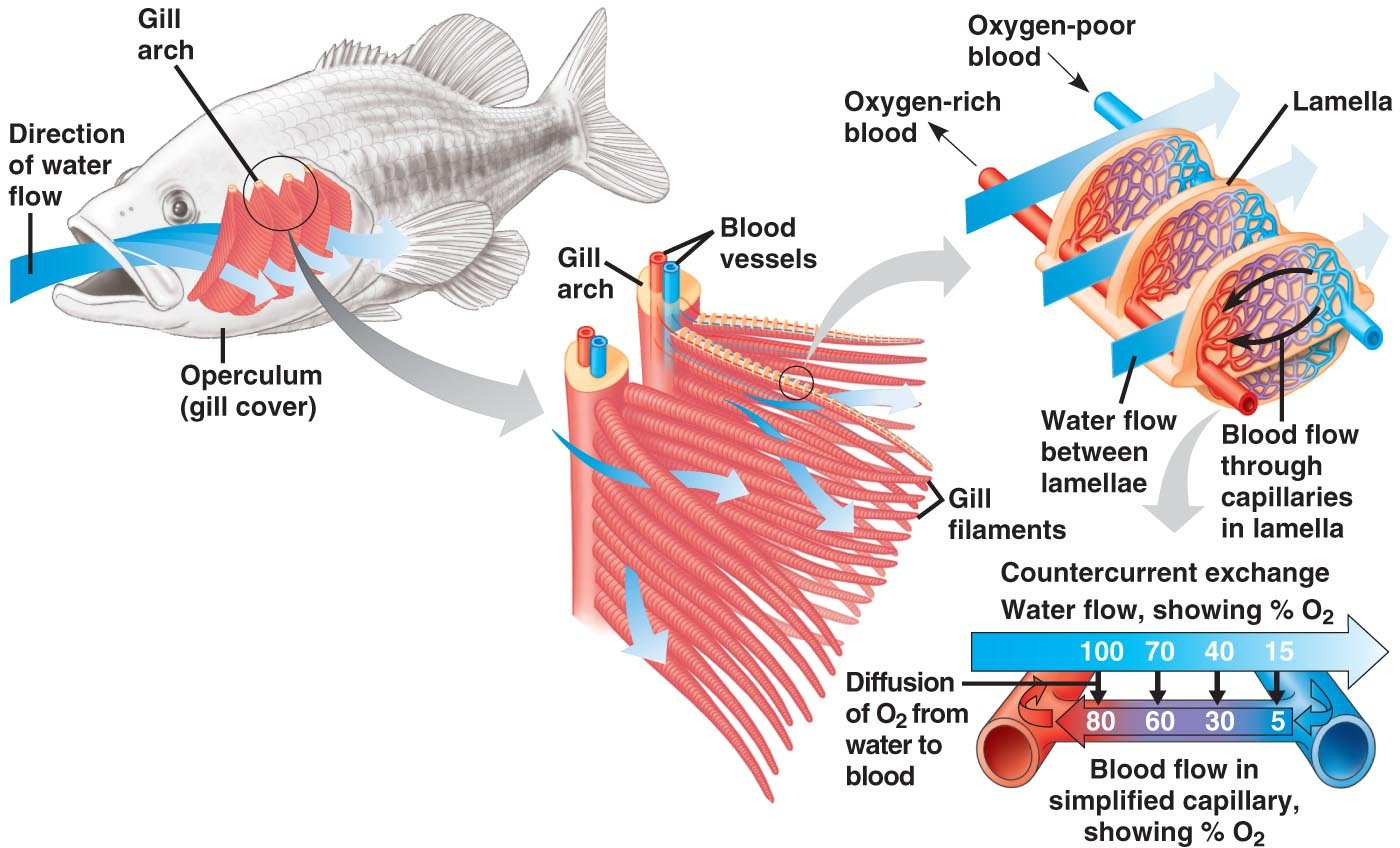
\includegraphics[width=0.618\linewidth]{./img/gills-an-o2}%
	\source{Campbell Biology}{\cite{Taylor2017}}
\end{frame}

\begin{frame}
	\frametitle{Gill anatomy}
	\begin{tikzpicture}[remember picture,overlay]%
		\node at (current page.center){%
			\animategraphics[autoplay,width=\paperwidth,every=\everyframe]{24}{./mov/fishhead/head-without-gills0}{001}{160}%
			};%
	\end{tikzpicture}%
\end{frame}

\begin{frame}
	\frametitle{Gill anatomy}
	\begin{tikzpicture}[remember picture,overlay]%
		\node at (current page.center){%
			\animategraphics[autoplay,width=\paperwidth,every=\everyframe]{24}{./mov/fishhead/head-without-gills0}{161}{481}%
			};%
	\end{tikzpicture}%
\end{frame}

\begin{frame}
	\frametitle{How?}
	\begin{columns}
		\begin{column}{0.5\linewidth}
				\begin{itemize}
					\item<1-> Training for \SI{5}{w}, \SI{5}{\day\per w}, \SI{6}{\hour\per\day}, at \SI{66}{\percent} of critical speed~\cite{Palstra2010}%
					\item<3-> Critical point drying%
					\item<4-> \uct imaging%
					\item<5-> Delineation in CTAn%
					\item<6-> Image analysis~\cite{Haberthur2019a}%
					\begin{itemize}
						\item<6-> Gill volume, structure and complexity%
					\end{itemize}
				\end{itemize}
		\end{column}
		\begin{column}{0.5\linewidth}
			\centering
				\only<1>{%
					\pgfmathsetlength{\imagewidth}{\imsize}%
					\pgfmathsetlength{\imagescale}{\imagewidth/1080}%
					\def\x{667}% scalebar-x starting at golden ratio of image width of 1080px = 667
					\def\y{547}% scalebar-y at 90% of image height of 608px = 547
					\begin{tikzpicture}[x=\imagescale,y=-\imagescale]%
						\node[anchor=north west, inner sep=0pt, outer sep=0pt] at (0,0) {\includegraphics[width=\imagewidth]{./mov/fishvideo/{{fishvideo_0033}}}};%
						% 69px = 30mm > 100px = 44mm > 1142px = 500mm, 228px = 100mm
						%\draw[|-|,blue] (410,188) -- (478,182) node [sloped,midway,above,fill=white,semitransparent,text opacity=1] {\SI{30}{\milli\meter} (TEMPORARY)};
						\draw[|-|,white] (\x,\y) -- (\x+228.4,\y) node [midway,above] {\(\approx\)\SI{10}{\centi\meter}};%
					\end{tikzpicture}%
					}%
				\only<2>{%
					% If you don't have the frames for the video, you can generate them as specified in ./mov/fishvideo/README.md
					\animategraphics[loop,autoplay,width=\imsize,every=\everyframe]{25}{./mov/fishvideo/fishvideo_0}{001}{250}%
					}%
				\only<3>{%
					\pgfmathsetlength{\imagewidth}{\imsize}%
					\pgfmathsetlength{\imagescale}{\imagewidth/1080}%
					\def\x{667}% scalebar-x starting at golden ratio of image width of 1080px = 667
					\def\y{673}% scalebar-y at 90% of image height of 748px = 673
					\def\shadow{4}% shadow parameter for scalebar
					\begin{tikzpicture}[x=\imagescale,y=-\imagescale]%
						\node[anchor=north west, inner sep=0pt, outer sep=0pt] at (0,0) {\includegraphics[height=0.618\textheight]{./img/{{IMG_20190603_174659}}}};%
						% 294px = 12.5mm > 100px = 4250um > 118px = 5mm
						%\draw[|-|,blue,thick] (494,218) -- (624,481) node [sloped,midway,above,fill=white,semitransparent,text opacity=1] {\SI{12.5}{\milli\meter} (294px) TEMPORARY!};
						\draw[|-|] (\x+\shadow,\y+\shadow) -- (\x+118+\shadow,\y+\shadow) node [midway, above] {\SI{5}{\milli\meter}};%
						\draw[|-|,white] (\x,\y) -- (\x+118,\y) node [midway,above] {\SI{5}{\milli\meter}};%
					\end{tikzpicture}%
					}%
				\only<4>{%
					\lstinputlisting[linerange={2-5,17-17,19-23,29-31,34-34,38-40,51-51,58-59}]{./logfiles/Control05/proj/Control05.log}%
					}%
				\only<5>{%
					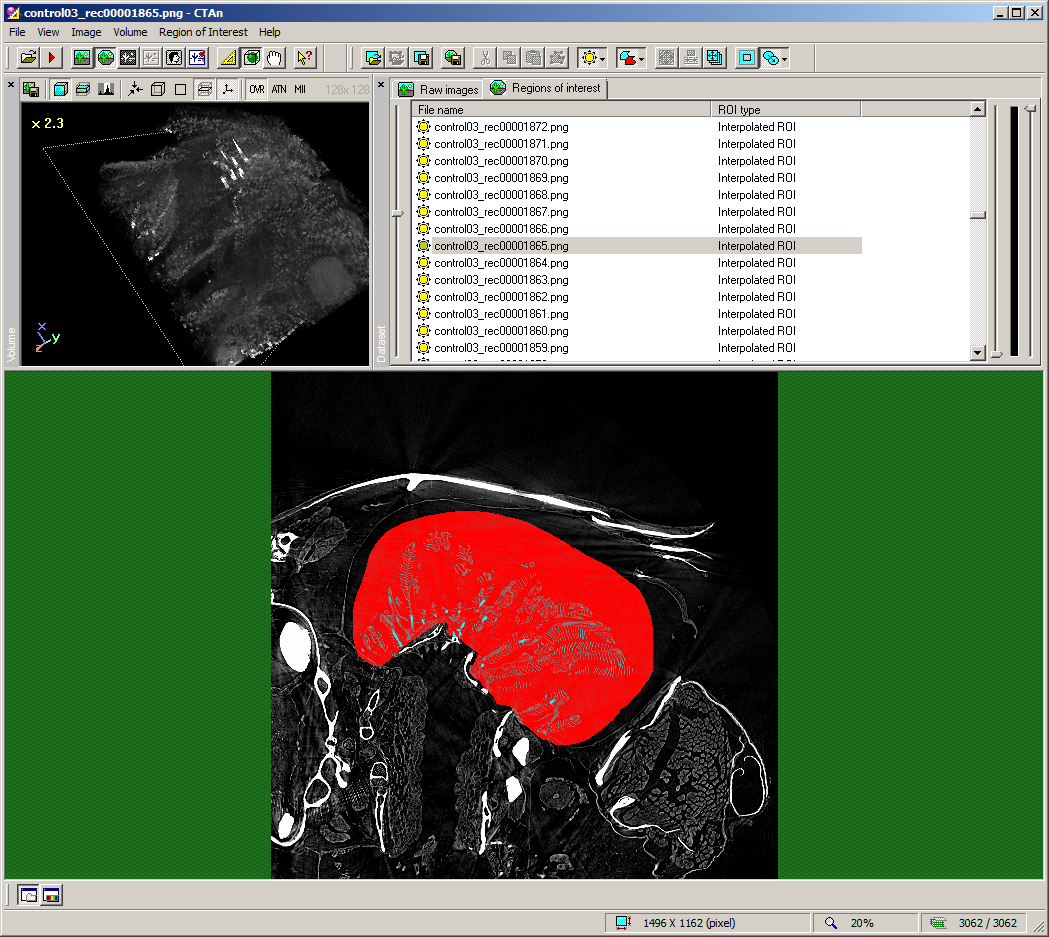
\includegraphics[height=0.618\textheight]{./img/CTAn}%
					}%
				\only<6>{%
					% If you don't have the frames for the video, you can generate them as specified in ./mov/coder/README.md
					\animategraphics[loop,autoplay,width=\imsize,every=\everyframe]{25}{./mov/coder/coder-}{0}{133}%
					\source{gph.is/2nqkple}{}%
					}%
		\end{column}
	\end{columns}
\end{frame}
\note{Comparable with the weekly training routine of Michael Phelps.
	The fish trained only for ca. \SI{7}{\percent} of their lifetime and started as adults.
	The Olympic winner trained for half of his lifetime and started as child.}

\begin{frame}
	\frametitle{Gill volume}
	\centering
	\only<1>{%
		\pgfmathsetlength{\imagewidth}{0.4\linewidth}%
		\pgfmathsetlength{\imagescale}{\imagewidth/2524}%
		\def\x{1560}% scalebar-x starting at golden ratio of image width of 2524px = 1560
		\def\y{2272}% scalebar-y at 90% of image height of 2524px = 2272
		\def\shadow{4}% shadow parameter for scalebar
		\begin{tikzpicture}[x=\imagescale,y=-\imagescale]
			\node[anchor=north west, inner sep=0pt, outer sep=0pt] at (0,0) {\includegraphics[width=\imagewidth]{./img/{{Control03_rec00001865}}}};
			% 2524px = 4.1874422mm > 100px = 166um > 301px = 500um, 60px = 100um
			%\draw[|-|,blue] (0,1262) -- (2524,1262) node [sloped,midway,above,fill=white,semitransparent,text opacity=1] {\SI{4.18}{\milli\meter} (2524px) TEMPORARY!};
			\draw[|-|] (\x+\shadow,\y+\shadow) -- (\x+301+\shadow,\y+\shadow) node [midway,above] {\SI{500}{\micro\meter}};
			\draw[|-|,white] (\x,\y) -- (\x+301,\y) node [midway,above] {\SI{500}{\micro\meter}};
		\end{tikzpicture}%
	}%
	\pgfmathsetlength{\imagewidth}{0.618\linewidth}%
	\pgfmathsetlength{\imagescale}{\imagewidth/2163}%
	\def\x{1730}% scalebar-x starting at golden ratio of image width of 2163px = 1337
	\def\y{1191}% scalebar-y at 90% of image height of 1323px = 1191
	\def\shadow{4}% shadow parameter for scalebar
	\only<2>{%
		\begin{tikzpicture}[x=\imagescale,y=-\imagescale]
			\node[anchor=north west, inner sep=0pt, outer sep=0pt] at (0,0) {\includegraphics[width=\imagewidth]{./img/{{Control03_rec00001865.crop}}}};
			% 2163px = 3.5885251499999997mm > 100px = 166um > 301px = 500um, 60px = 100um
			\draw[|-|] (\x+\shadow,\y+\shadow) -- (\x+301+\shadow,\y+\shadow) node [midway,above] {\SI{500}{\micro\meter}};
			\draw[|-|,white] (\x,\y) -- (\x+301,\y) node [midway,above] {\SI{500}{\micro\meter}};
		\end{tikzpicture}%
		}%
	\only<3>{%
		\begin{tikzpicture}[x=\imagescale,y=-\imagescale]
			\node[anchor=north west, inner sep=0pt, outer sep=0pt] at (0,0) {\includegraphics[width=\imagewidth]{./img/{{control03_rec0000_voi_1865.crop}}}};
			\draw[|-|] (\x+\shadow,\y+\shadow) -- (\x+301+\shadow,\y+\shadow) node [midway,above] {\SI{500}{\micro\meter}};
			\draw[|-|,white] (\x,\y) -- (\x+301,\y) node [midway,above] {\SI{500}{\micro\meter}};
		\end{tikzpicture}%
		}%
	\only<4>{%
		\begin{tikzpicture}[x=\imagescale,y=-\imagescale]
			\node[anchor=north west, inner sep=0pt, outer sep=0pt] at (0,0) {\includegraphics[width=\imagewidth]{./img/{{Control03_thresholded_1500.crop}}}};
			\draw[|-|] (\x+\shadow,\y+\shadow) -- (\x+301+\shadow,\y+\shadow) node [midway,above] {\SI{500}{\micro\meter}};
			\draw[|-|,white] (\x,\y) -- (\x+301,\y) node [midway,above] {\SI{500}{\micro\meter}};
		\end{tikzpicture}%
		}%
	\only<5>{% !TEX root = ..\20190605_BrukerUserMeeting.tex
% This file was created by matplotlib2tikz v0.7.4.
% And edited a bit by hand...
\begin{tikzpicture}

%\definecolor{color0}{rgb}{0.83921568627451,0,0.168627450980392}

\begin{axis}[
simplified,
scale only axis,
width=0.75\textwidth,
height=.618\textheight,
%axis line style={white!80.0!black},
%tick align=outside,
%x grid style={white!80.0!black},
%xmajorticks=false,
%xmin=-0.5, xmax=1.5,
%xtick style={color=white!15.0!black},
xtick={0,1},
xticklabels={Control,Swimmer},
%y grid style={white!80.0!black},
ylabel={Gill volume [\si{\micro\litre}]},
%ymajorgrids,
%ymajorticks=false,
%ymin=0, %ymax=0.770697055458566,
%ytick style={color=white!15.0!black},
%ytick={0,0.1,0.2,0.3,0.4,0.5,0.6,0.7},
%yticklabels={0.0,0.1,0.2,0.3,0.4,0.5,0.6,0.7}
]
\path [draw=black, fill=lightgray]
(axis cs:-0.4,0.447649695726768)
--(axis cs:0.4,0.447649695726768)
--(axis cs:0.4,0.554668101627052)
--(axis cs:-0.4,0.554668101627052)
--(axis cs:-0.4,0.447649695726768)
--cycle;
\path [draw=black, fill=ubRed]
(axis cs:0.6,0.486075630595014)
--(axis cs:1.4,0.486075630595014)
--(axis cs:1.4,0.58742018834191)
--(axis cs:0.6,0.58742018834191)
--(axis cs:0.6,0.486075630595014)
--cycle;
\addplot [black]
table {%
0 0.447649695726768
0 0.376938425845528
};
\addplot [black]
table {%
0 0.554668101627052
0 0.572242192769256
};
\addplot [black]
table {%
-0.2 0.376938425845528
0.2 0.376938425845528
};
\addplot [black]
table {%
-0.2 0.572242192769256
0.2 0.572242192769256
};
\addplot [black]
table {%
1 0.486075630595014
1 0.427215702498488
};
\addplot [black]
table {%
1 0.58742018834191
1 0.623046643313328
};
\addplot [black]
table {%
0.8 0.427215702498488
1.2 0.427215702498488
};
\addplot [black]
table {%
0.8 0.623046643313328
1.2 0.623046643313328
};
%\addplot [black, mark=x, mark size=2, mark options={solid,fill=white!25.098039215686274!black}, only marks]
%table {%
%1 0.749298475419024
%};
\addplot [black]
table {%
-0.4 0.48488362116854
0.4 0.48488362116854
};
\addplot [black]
table {%
0.6 0.542154490975104
1.4 0.542154490975104
};
\addplot [only marks, draw=black, fill=lightgray]
table{%
x                      y
0.118169013092897 0.572242192769256
0.10855628965999 0.471672297437017
0.150748883239949 0.56475262570696
0.0405875827483924 0.568003444252336
0.0798225109401674 0.524414529387328
-0.0441479545054979 0.484753900995424
-0.110657373100773 0.376938425845528
0.0923901849786244 0.439642161823352
-0.0508500091298818 0.41752174920648
-0.0881348920135038 0.485013341341656
};
\addplot [only marks, draw=black, fill=ubRed]
table{%
x                      y
0.971381935247385 0.567564796770337
0.807508339276123 0.503736968660552
1.16935274550397 0.449384355640976
0.927163647331323 0.480188517906501
0.956312477868329 0.623046643313328
1.09621385012237 0.577596442831624
1.09835666014502 0.590694770178672
1.11931844258053 0.516744185179872
1.12159157456604 0.749298475419024
1.01159718977894 0.427215702498488
};
\draw[|-|, thin, gray] (axis cs:1,0.756791460173214) -- (axis cs:0,0.756791460173214) node [midway,above] {\scriptsize * | p=\num{0.048}};
%\draw[] (axis cs:0.5,0.756791460173214) -- (axis cs:0.5,0.756791460173214);
%\node at (axis cs:0.5,0.756791460173214)[
%  scale=0.9,
%  fill=lightgray,
%  draw=black,
%  line width=0.6pt,
%  inner sep=2.2pt,
%  text=black,
%  rotate=0.0
%]{* | p=0.048};
\end{axis}

\end{tikzpicture}}
\end{frame}
\note{We analyzed 20 samples with a mean size of a cube with a side length of 1863 pixels.
	This means we analyzed 129.40 GigaPixels.
	This means we analyzed \num{129395.29} MegaPixels.
	In total \num{46014} slices.}

\begin{frame}
	\frametitle{Gill complexity}
	\centering
	\pgfmathsetlength{\imagewidth}{0.618\linewidth}%
	\pgfmathsetlength{\imagescale}{\imagewidth/2163}%
	\def\x{1730}% scalebar-x starting at golden ratio of image width of 2163px = 1337
	\def\y{1191}% scalebar-y at 90% of image height of 1323px = 1191
	\def\shadow{4}% shadow parameter for scalebar
	\only<1>{%
		\begin{tikzpicture}[x=\imagescale,y=-\imagescale]
			\node[anchor=north west, inner sep=0pt, outer sep=0pt] at (0,0) {\includegraphics[width=\imagewidth]{./img/{{Control03_thresholded_1500.crop}}}};
			\draw[|-|] (\x+\shadow,\y+\shadow) -- (\x+301+\shadow,\y+\shadow) node [midway,above] {\SI{500}{\micro\meter}};
			\draw[|-|,white] (\x,\y) -- (\x+301,\y) node [midway,above] {\SI{500}{\micro\meter}};
		\end{tikzpicture}%
		}%
	\only<2>{%
		\begin{tikzpicture}[x=\imagescale,y=-\imagescale]
			\node[anchor=north west, inner sep=0pt, outer sep=0pt] at (0,0) {\includegraphics[width=\imagewidth]{./img/{{Control03_area_organ_1500.crop.edit}}}};
			\draw[|-|] (\x+\shadow,\y+\shadow) -- (\x+301+\shadow,\y+\shadow) node [midway,above] {\SI{500}{\micro\meter}};
			\draw[|-|,white] (\x,\y) -- (\x+301,\y) node [midway,above] {\SI{500}{\micro\meter}};
		\end{tikzpicture}%
		}%
	\only<3>{%
		\begin{tikzpicture}[x=\imagescale,y=-\imagescale]
			\node[anchor=north west, inner sep=0pt, outer sep=0pt] at (0,0) {\includegraphics[width=\imagewidth]{./img/{{Control03_area_organ_1500.crop.combination}}}};
			\draw[|-|] (\x+\shadow,\y+\shadow) -- (\x+301+\shadow,\y+\shadow) node [midway,above] {\SI{500}{\micro\meter}};
			\draw[|-|,white] (\x,\y) -- (\x+301,\y) node [midway,above] {\SI{500}{\micro\meter}};
		\end{tikzpicture}%
		}%
	\only<4>{%
		\begin{tikzpicture}[remember picture,overlay]%
			\node at (current page.center){%
				\animategraphics[palindrome,autoplay,width=\paperwidth,every=\everyframe]{25}{./mov/complexity/control03_thresholded_0}{025}{256}%
				};%
		\end{tikzpicture}%
		}%
	\only<5>{% !TEX root = ..\20190605_BrukerUserMeeting.tex
% This file was created by matplotlib2tikz v0.7.4.
% And edited a bit by hand...
\begin{tikzpicture}

%\definecolor{color0}{rgb}{0.83921568627451,0,0.168627450980392}

\begin{axis}[
simplified,
scale only axis,
width=0.75\textwidth,
height=.618\textheight,
%axis line style={white!80.0!black},
%tick align=outside,
%x grid style={white!80.0!black},
%xlabel={Experiment},
%xmajorticks=false,
%xmin=-0.5, xmax=1.5,
%xtick style={color=white!15.0!black},
xtick={0,1},
xticklabels={Control,Swimmer},
%y grid style={white!80.0!black},
ylabel={Gills per organ [\si{\percent}]},
%ymajorgrids,
%ymajorticks=false,
%ymin=0,
ymax=0.45,
yticklabel={\pgfmathparse{\tick*100}\pgfmathprintnumber{\pgfmathresult}}, % percentage instead of value: https://tex.stackexchange.com/a/87431/828
%ytick style={color=white!15.0!black},
%ytick={0,0.05,0.1,0.15,0.2,0.25,0.3,0.35,0.4},
%yticklabels={0.00,0.05,0.10,0.15,0.20,0.25,0.30,0.35,0.40}
]
\path [draw=black, fill=lightgray]
(axis cs:-0.4,0.382496841309432)
--(axis cs:0.4,0.382496841309432)
--(axis cs:0.4,0.40078453974052)
--(axis cs:-0.4,0.40078453974052)
--(axis cs:-0.4,0.382496841309432)
--cycle;
\path [draw=black, fill=ubRed]
(axis cs:0.6,0.349508101341073)
--(axis cs:1.4,0.349508101341073)
--(axis cs:1.4,0.367828846032819)
--(axis cs:0.6,0.367828846032819)
--(axis cs:0.6,0.349508101341073)
--cycle;
\addplot [black]
table {%
0 0.382496841309432
0 0.366846367137451
};
\addplot [black]
table {%
0 0.40078453974052
0 0.421306108182572
};
\addplot [black]
table {%
-0.2 0.366846367137451
0.2 0.366846367137451
};
\addplot [black]
table {%
-0.2 0.421306108182572
0.2 0.421306108182572
};
%\addplot [black, mark=x, mark size=2, mark options={solid,fill=white!25.098039215686274!black}, only marks]
%table {%
%0 0.324346236114214
%0 0.430803679704798
%};
\addplot [black]
table {%
1 0.349508101341073
1 0.328636765492142
};
\addplot [black]
table {%
1 0.367828846032819
1 0.370980682541585
};
\addplot [black]
table {%
0.8 0.328636765492142
1.2 0.328636765492142
};
\addplot [black]
table {%
0.8 0.370980682541585
1.2 0.370980682541585
};
%\addplot [black, mark=x, mark size=2, mark options={solid,fill=white!25.098039215686274!black}, only marks]
%table {%
%1 0.397507730617411
%};
\addplot [black]
table {%
-0.4 0.385498429400225
0.4 0.385498429400225
};
\addplot [black]
table {%
0.6 0.359924925696058
1.4 0.359924925696058
};
\addplot [only marks, draw=black, fill=lightgray]
table{%
x                      y
0.122760548828477 0.398180638009362
0.178377085421143 0.384645825823707
0.0632274378419731 0.385682004675644
-0.194111991081275 0.381780513138006
-0.197119839709041 0.401652506984239
0.17337636979033 0.430803679704798
0.0108063396631302 0.421306108182572
0.128021270524512 0.324346236114214
-0.00795828164448514 0.366846367137451
0.139091086002659 0.385314854124806
};
\addplot [only marks, draw=black, fill=ubRed]
table{%
x                      y
1.0151048710241 0.360517193679055
0.937200439503442 0.363812777627831
1.02779049814574 0.328636765492142
1.11423867280775 0.35933265771306
1.07668523249001 0.330896994967363
0.859861308304989 0.346290741881158
0.883487590339555 0.397507730617411
0.818543013016209 0.370980682541585
0.802416546522818 0.359160179720818
1.17448234469223 0.369167535501148
};
\draw[|-|, thin, gray] (axis cs:1,0.435111716501846) -- (axis cs:0,0.435111716501846) node [midway,above] {\scriptsize ** | p=\num{0.0088}};
%\draw[] (axis cs:0.5,0.435111716501846) -- (axis cs:0.5,0.435111716501846);
%\node at (axis cs:0.5,0.435111716501846)[
%  scale=0.9,
%  fill=lightgray,
%  draw=black,
%  line width=0.6pt,
%  inner sep=2.2pt,
%  text=black,
%  rotate=0.0
%]{** | p=0.0088};
\end{axis}

\end{tikzpicture}}
\end{frame}

\begin{frame}
	\frametitle{Thanks!}
	\begin{columns}
		\begin{column}{0.5\linewidth}
		\begin{itemize}
			\item Topographic and clinical Anatomy
			\begin{itemize}
				\item Valentin Djonov, Ruslan Hlushchuk
				\item Dea Aaldijk, Matthias Messerli
				\item Fluri Wieland, Oleksiy-Zakhar Khoma
				\item Sarya Fark, Helena Röss
			\end{itemize}
			\item Fish facility team
			\begin{itemize}
				\item<1-> Regula Buergy, Eveline Yao and Sara Soltermann
				\item<1-> Ines Marquez, Xavier Langa and Alexander Uwe Ernst
			\end{itemize}
			\item SNF
			\item<2-> You, for listening!
			\item<3-> Questions?
		\end{itemize}
		\end{column}
		\begin{column}{0.5\linewidth}
			\includegraphics<1->[height=.7\textheight]{./img/team}
		\end{column}
	\end{columns}
\end{frame}

\begin{frame}
	\frametitle{References}
	%\renewcommand*{\bibfont}{\scriptsize}
	\setbeamertemplate{bibliography item}{\insertbiblabel}
	\printbibliography
\end{frame}

\begin{frame}
	\frametitle{Colophon}
	\begin{itemize}
		\item \href{https://github.com/habi/Talk.2019.MicroCTWorkshop}{The presentation (\LaTeX/\textsc{beamer}) is available on GitHub}: git.io/Je4oh
		\item \href{https://github.com/habi/Zebra-Fish-Gills/}{The full analysis of the data (\faPython) is also available on GitHub}: git.io/fjuoF\newline
			Details are described in~\cite{Messerli2019a}: 
		\item \href{http://intern.unibe.ch/dienstleistungen/corporate_design_und_vorlagen/praesentationen/index_ger.html}{The presentation template is from \emph{Corporate Design und Vorlagen, University of Bern}}
	\end{itemize}
\end{frame}

\end{document}
